%%%%%%%%%%%%%%%%%%%%%%%%%%%%%%%%%%%%%%%%%%%%%%%%%%
%	JASA LaTeX Template File
%  For use in making articles using JASAnew.cls
% July 26, 2017
%%%%%%%%%%%%%%%%%%%%%%%%%%%%%%%%%%%%%%%%%%%%%%%%%%

%% Step 1:
%% Uncomment the style that you want to use:

%%%%%%% For Preprint
%% For manuscript, 12pt, one column style

%% Comment this out if you'd rather use another style:
\documentclass[preprint]{JASAnew}

%%%%% Preprint Options %%%%%
%% The track changes option allows you to mark changes
%% and will produce a list of changes, their line number
%% and page number at the end of the article.
%\documentclass[preprint,trackchanges]{JASAnew}

%% authaffil option will make affil immediately
% follow author, otherwise authors are grouped, and affiliations
% are stacked underneath all the authors.
%\documentclass[preprint,authaffil]{JASAnew}

%% NumberedRefs is used for numbered bibliography and citations.
%% Default is Author-Year style.
%% \documentclass[preprint,NumberedRefs]{JASAnew}

%%%%%%% For Reprint
%% For appearance of finished article; 2 columns, 10 pt fonts

% \documentclass[reprint]{JASAnew}

%%%%% Reprint Options %%%%%

%% For testing to see if author has exceeded page length request, use 12pt option
%\documentclass[reprint,12pt]{JASAnew}

% authaffil option will make affil immediately
% follow author, otherwise authors are grouped, and affiliations
% are stacked underneath all the authors.
%\documentclass[reprint,authaffil]{JASAnew}

%% NumberedRefs is used for numbered bibliography and citations.
%% Default is Author-Year style.
% \documentclass[reprint,NumberedRefs]{JASAnew}

%% TurnOnLineNumbers
%% Make lines be numbered in reprint style:
% \documentclass[reprint,TurnOnLineNumbers]{JASAnew}

\usepackage{fontspec}

    \setmainfont[StylisticSet=20,Numbers=Lining]{Brill}

\usepackage{natbib}


\let\tnote\relax
\usepackage{cleveref}
\usepackage{ctable}

\begin{document}
%% the square bracket argument will send term to running head in
%% preprint, or running foot in reprint style.

\title[]{Longer vowel duration correlates with greater tongue root displacement:
Acoustic and articulatory data from Italian and Polish}

% ie
%\title[JASA/Sample JASA Article]{Sample JASA Article}

%% repeat as needed

\author{Stefano Coretta}
% ie
%\affiliation{Department1,  University1, City, State ZipCode, Country}
\affiliation{Linguistics and English Language, University of Manchester, Oxford Road,
Manchester, M13 9PL, United Kingdom}
%% for corresponding author
\email{stefano.coretta@manchester.ac.uk}
%% for additional information


% ie
% \author{Author Four}
% \email{author.four@university.edu}
% \thanks{Also at Another University, City, State ZipCode, Country.}

%% For preprint only,
%  optional, if you want want this message to appear in upper left corner of title page
% \preprint{}

%ie
%\preprint{Author, JASA}

% optional, if desired:
%\date{\today}

\begin{abstract}
% Put your abstract here. Abstracts are limited to 200 words for
% regular articles and 100 words for Letters to the Editor. Please no
% personal pronouns, also please do not use the words ``new'' and/or
% ``novel'' in the abstract. An article usually includes an abstract, a
% concise summary of the work covered at length in the main body of the
% article.
Voiced stops tend to be preceded by longer vowels and produced with a
more advanced tongue root than voiceless stops. The duration of a vowel
is modulated by the voicing of the stop that follows and in many
languages vowels are longer when followed by voiced stops. Tongue root
advancement is known to be an articulatory mechanism which ensures the
right pressure conditions for the maintenance of voicing during closure
as dictated by the Aerodynamic Voicing Constraint. In this paper, it is
argued that vowel duration and tongue root advancement enter in a direct
statistical relation. Drawing from acoustic and ultrasound tongue
imaging data from 17 speakers of Italian and Polish, it is shown that
tongue root advancement is initiated during the vowel, and that vowel
duration and tongue root position at vowel offset are positively
correlated. Longer vowel durations correspond to greater tongue root
advancement. It is further proposed that the later closure onset of
voiced stops within a temporally stable interval is responsible for both
greater root advancement and shorter closure durations in the context of
voiced stops.
\end{abstract}

%% pacs numbers not used

\maketitle

%  End of title page for Preprint option --------------------------------- %

%% See preprint.tex/.pdf or reprint.tex/.pdf for many examples


%  Body of the article
\hypertarget{introduction}{%
\section{Introduction}\label{introduction}}

It is well known that voiced stops are almost universally characterised
by two phonetic correlates: advanced tongue root and increased duration
of the preceding vowel \citep{westbury1983, lisker1974, fowler1992}.
While a lot of work has been done on each of these aspects separately,
less is known about their relation. In this paper, I propose a link
between the position of the tongue root at the onset of a post-vocalic
stop and the duration of the vowel preceding that stop. In an
exploratory study of the articulatory correlates of stop voicing, it was
found that tongue root advancement---a mechanism known to facilitate
voicing during stop closure---is initiated during the production of the
vowel preceding the stop. This replicates previous work on tongue root
position. Furthermore, the results of this study indicate that the
acoustic duration of the vowel is positively correlated with tongue root
position, such that longer vowel durations correspond to greater tongue
root advancement. Such correlation is shown to derive from the timing of
the consonantal closure relative to the preceding vowel.

\hypertarget{tongue-root-position-and-voicing}{%
\subsection{Tongue root position and
voicing}\label{tongue-root-position-and-voicing}}

One of the differences in supra-glottal articulation between voiced and
voiceless stops concerns the position of the tongue root relative to the
front-back dimension of the oral tract. It has been repeatedly observed
that the tongue root is in a more front position in voiced stops
compared to voiceless stops \citep{kent1969, perkell1969, westbury1983}.
This has been attributed to the fact that the initiation and maintenance
of vocal fold vibration (i.e.~voicing) requires a difference in air
pressure between the cavities below and above the glottis. Specifically,
the sub-glottal pressure needs to be higher than the supra-glottal
pressure. In other words, there must be a positive trans-glottal air
pressure differential \citep{berg1958, rothenberg1967}. This property of
voicing is formally known as the Aerodynamic Voicing Constraint
\citep{ohala2011}. When the oral tract is completely occluded during the
production of a stop closure, the supra-glottal pressure quickly
increases, due to the incoming airstream from the lungs. Such pressure
increase can hinder the ability to sustain vocal fold vibration during
closure, to the point voicing ceases.

An articulatory solution to counterbalance the increased pressure is to
enlarge the supra-glottal cavity by advancing the root of the tongue. In
the context of articulatory adjustments, a distinction between passive
and active gestures is generally drawn (see for example
\citealt{rothenberg1967}). A passive enlargement of the oral cavity is
the product of the incoming airflow, the pressure of which expands the
pliable soft tissues of the cavity walls. On the other hand, active
expansion is achieved by muscular activity, which can in turn be
purposive (produced with the goal of cavity expansion) or non-purposive.
While \citet{rothenberg1967} recognises that the distinction between
purposive and non-purposive active gestures can be at times blurry, it
is nonetheless important to note that the qualification of a gesture as
active does not automatically implies a speaker's intention to produce
the obtained result.

\citet{rothenberg1967} further calculates that the walls of the oral
tract can absorb the incoming airflow for 20 to 30 ms by passive
expansion, after which the sub- and supra-glottal pressures would
equalise and voicing cease. Based on these estimates, a passive
expansion of the pharyngeal walls is thus not generally sufficient to
maintain voicing during the closure of a stop. Reaching a complete
ballistic forward gesture would require the tongue root about 70 to 90
ms \citep{rothenberg1967}. Given that voiced stop closures are on
average shorter than that (the mean duration is about 64 ms in
\citealt{luce1985}), it is expected that the movement could be initiated
during the production of the vowel, so that an appreciable amount of
advancement is obtained when closure is achieved. Furthermore,
\citet{westbury1983} finds that tongue root advancement is initiated
before the achievement of full closure and that there is a forward
movement even in some cases of voiceless stops, although the rate and
magnitude of the advancement are consistently higher in voiced stops.
Finally, tongue root adjustments seem to target more specifically
lingual consonants, while the tongue body is more involved in labials
\citep{perkell1969, westbury1983}.

However, the relation between tongue root advancement and voicing is a
complex one. First, tongue root advancement is not the only mechanism
for sustaining voicing during a stop
\citep{rothenberg1967, westbury1983, ohala2011} and it has a certain
degree of idiosyncrasy \citep{ahn2018}. For example, a
cross-lingusitically common difference between voiceless and voiced
stops concerns their respective closure durations. The closure of voiced
stops is generally longer than that of voiceless stops
\citep{lisker1957, umeda1977, van-summers1987, davis1989, de-jong1991}.
A shorter closure favours maintenance of vocal fold vibration by
ensuring that the pressure build-up in the oral cavity does not equalise
the sub-glottal and supra-glottal pressures (at which point voicing
would stop). Other solutions which can help sustaining voicing during
closure include larynx lowering \citep{riordan1980}, slackening of the
vocal folds \citet{halle1967}, opening of the velopharyngeal port
\citep{yanagihara1966}, and producing a retroflex occlusion
\citep{sprouse2008}. Moreover, \citep{ahn2018} finds that not all the
speakers she surveyed did show tongue root advancement, and a few had
rather the reverse pattern.

Second, implementation of tongue root advancement can be decoupled from
the actual presence of vocal fold vibration. In \citet{westbury1983},
advancement of the tongue root is found in some productions of voiceless
stops. This is counterintuitive, since tongue root advancement is
generally considered to be a feature of voiced stops which require
voicing-related pressure adjustments. Moreover, \citet{ahn2015, ahn2018}
and \citet{ahn2016} looked at utterance-initial stops and found that the
tongue root is more advanced in the phonologically voiced stops
independent of whether they are implemented with vocal fold vibration or
not.

To summarise, tongue root advancement is a common articulatory solution
employed to counterbalance the increase in supra-glottal pressure and
maintaining voicing during the production of at least lingual voiced
stops. While this gesture is not exclusive of voiced stops and it can be
implemented even in the absence of vocal fold vibration, tongue root
advancement seems to be a robust correlate of voicing.

\hypertarget{vowel-duration-and-voicing}{%
\subsection{Vowel duration and
voicing}\label{vowel-duration-and-voicing}}

The results discussed here are part of a larger study which focusses on
the effect of consonant voicing on preceding vowel durations. A great
number of studies showed that, cross-linguistically, vowels tend to be
longer when followed by voiced obstruents than when they are followed by
voiceless ones
\citep{house1953, peterson1960, chen1970, klatt1973, lisker1974, farnetani1986, fowler1992, hussein1994, esposito2002, lampp2004, durvasula2012}.
This so-called `voicing effect' has been reported in a variety of
languages, including (but not limited to) English, German, Hindi,
Russian, Arabic, Korean, Italian, and Polish (see
\citealt{maddieson1976} and \citealt{begus2017} for a more comprehensive
list).

Italian and Polish offer an opportunity to study of the articulatory
aspects of the voicing effect, given their reported differences in
magnitude/presence of the effect and the relative ease of comparison.
While Italian has been consistently reported as a voicing-effect
language \citep{caldognetto1979, farnetani1986, esposito2002}, some
studies found an effect in Polish
\citep{slowiaczek1985, nowak2006, malisz2008, coretta2018j} while others
did not \citep{keating1984, jassem1989}.

\citet{coretta2018j} argues, based on the acoustics of the same data
reported here, that the stressed vowels of disyllabic (CV́CV) words in
Italian and Polish are 16 ms longer (SE = 4.4) when followed by a voiced
stop. The high degree of intra-speaker variation, backed up by
statistical modelling, also indicates that these languages possibly
behave similarly in regards to the voicing effect. Finally, the temporal
distance between two consecutive stop releases in CV́CV words is not
affected by the voicing of the second consonant. The duration of the
release to release interval is stable across voicing contexts. Within
this interval, the timing of VC boundary (the vowel offset/onset of stop
closure) produces differences in the respective durations of vowel and
closure, following a mechanism of temporal compensation
\citep{lindblom1967, slis1969a, slis1969, lehiste1970, lehiste1970a}. A
later closure onset results in a long vowel and a short closure, while
an earlier closure onset corresponds to a short vowel and a long
closure. Since the closure of voiceless stops is longer than that of
voiced stops, it follows that vowels are shorter when followed by the
former than when followed by the latter.

\hypertarget{this-study}{%
\subsection{This study}\label{this-study}}

Previous research has established that tongue root advancement and
longer vowel durations are two common correlates of voicing. In
particular, voicing during closure can be maintained by advancing the
tongue root during the production of voiced stops (which is possibly
initiated earlier than the closure onset) and that vowels followed by
voiced stops tend to be longer than vowels followed by voiceless stops.
The acoustic data further revealed that the duration of the stop closure
bears on the duration of the preceding vowel, by means of a kind of
compensatory mechanism.

The results from the articulatory data of this study, which will be
discussed in the following sections, offer new insights on the link
between closure and vowel duration. We will see that the relative timing
of the closure also modulates the degree of tongue root advancement
found at closure onset, thus creating a three-way network of relations
with vowel duration and tongue root position. More specifically, the
timing of the closure onset within the release-to-release interval
decides the duration of the vowel, the duration of the closure, and the
degree of tongue root advancement. Finally, it will be argued that a
later closure onset as in the case of voiced stops has the double
advantage of producing both a short closure duration and greater tongue
root advancement, features both known to comply with the Aerodynamic
Voicing Constraint.

\hypertarget{methodology}{%
\section{Methodology}\label{methodology}}

Following recent practices which encourage scientific transparency and
data attribution \citep{cruwell2018, berez-kroeker2018, roettger2019},
data \citep{coretta2018m} and analysis code are available on the Open
Science
Framework.\footnote{The analysis code can be found at this temporary link for peer-review: \url{https://osf.io/d245b/?view_only=c7ec58d937454de8b7ad9212c261776b}. A public link will be generated in case of acceptance.}

\hypertarget{participants}{%
\subsection{Participants}\label{participants}}

Participants were recruited in Manchester (UK), and Verbania (Italy)
Eleven native speakers of Italian (5 females, 6 males) and 6 native
speakers of Polish (3 females, 3 males) participated in this study. Most
speakers of Italian are originally from the North of Italy, while 3 are
from Central Italy. The Polish speakers came from different parts of
Poland (2 from the west, 3 from the centre, and 1 from the east). This
study has been approved by the School of Arts, Languages, and Culture
Ethics committee of the University of Manchester (REF 2016-0099-76). The
participants signed a written consent and received a monetary
compensation of £10.

\hypertarget{equipment}{%
\subsection{Equipment}\label{equipment}}

\label{s:equipment}

Simultaneous recordings of audio and ultrasound tongue imaging were
obtained in the Phonetics Laboratory at the University of Manchester
(UK) or in a quiet room in Verbania (Italy). An Articulate Instruments
Ltd™ system was used for this study. The system is made of a TELEMED
Echo Blaster 128 unit, an Articulate Instruments Ltd™ P-Stretch
synchronisation unit, and a FocusRight Scarlett Solo pre-amplifier. A
TELEMED C3.5/20/128Z-3 ultrasonic transducer (20mm radius, 2-4 MHz) and
a Movo LV4-O2 Lavalier microphone were used respectively for the
acquisition of ultrasonic and audio data. The ultrasonic probe was
placed in contact with the sub-mental triangle, aligned with the
mid-sagittal plane. A metallic headset designed by Articulate
Instruments Ltd™ (\citeyear{articulate2008}) was used to hold the probe
in a fixed position and inclination relative to the head. The
acquisition of the mid-sagittal ultrasonic and audio signals was
achieved with the software Articulate Assistant Advanced (AAA, v2.17.2)
running on a Hewlett-Packard ProBook 6750b laptop with Microsoft Windows
7. The synchronisation of the ultrasonic and audio signals was performed
by AAA after recording by means of a synchronisation signal produced by
the P-Stretch unit. The ranges of the ultrasonic settings were: 43-68
frames per second, 88-114 number of scan lines, 980-988 pixel per scan
line, field of view 71-93°, pixel offset 109-263, depth 75-180 mm. The
audio signal was sampled at 22050 Hz (16-bit).

\hypertarget{materials}{%
\subsection{Materials}\label{materials}}

Disyllabic words of the form
C\textsubscript{1}V\textsubscript{1}C\textsubscript{2}V\textsubscript{2}
were used as targets, where C\textsubscript{1} = /p/, V\textsubscript{1}
= /a, o, u/, C\textsubscript{2} = /t, d, k, g/, and V\textsubscript{2} =
V\textsubscript{1} (e.g.~\emph{pata}, \emph{pada}, \emph{poto}, etc.),
giving a total of 12 target words, used both for Italian and
Polish.\footnote{Note that stressed vowels in open syllables in Italian are long \citep{renwick2016}. Moreover, /o/ is used here for typographical simplicity to indicate the mid-back vowels of Italian and Polish, although they do differ in quality. See \citet{kramer2009}, \citet{renwick2016}, and \citet{gussmann2007}.}
The resulting words are nonce words, with a few exceptions, and they
were presented in the languages' respective writing conventions (see
\Cref{a:targets}). A labial stop was chosen as the first consonant to
reduce possible coarticulation with the following
vowel.\footnote{However, note that \citet{westbury1983} and \citet{vazquez-alvarez2007} report tongue body lowering in the context of labial stops.}
Central/back vowels only were included in the target words for two
reasons. First, high and mid front vowels tend to be difficult to image
with ultrasound, given their greater distance from the ultrasonic probe
when compared with back vowels. Second, high and mid front vowels
usually produce less tongue displacement from and to a stop consonant.
This characteristic can make it more difficult to identify gestural
landmarks using the methodology discussed in \Cref{s:process}. Since the
focus of the study was to explore differences in the closing gesture of
voiceless and voiced stops, only lingual consonants have been included
(the closure of labial stops cannot of course be imaged with
ultrasound). The sentence \emph{Dico X lentamente} `I say X slowly' in
Italian, and \emph{Mówię X teraz} `I say X now' for Polish functioned as
frames for the test words. Speakers were instructed to read the
sentences without pauses and to speak at a comfortable pace.

\hypertarget{procedure}{%
\subsection{Procedure}\label{procedure}}

The participants familiarised themselves with the sentence stimuli at
the beginning of the session. Headset and probe were then fitted on the
participant's head. The participant read the sentence stimuli, which
were presented on the computer screen in a random order, while the audio
and ultrasonic signals were acquired simultaneously. The random list of
sentences was read 6 times consecutively (with the exception of IT02,
who repeated the sentences 5 times only). Due to software constraints,
the order of the sentences within participant was kept the same for each
of the six repetitions. The participant could optionally take breaks
between one repetition and the other. Sentences with hesitations or
speech errors were immediately discarded and re-recorded. A total of
1212 tokens (792 from Italian, 420 from Polish) were obtained.

\hypertarget{data-processing-and-statistical-analysis}{%
\subsection{Data processing and statistical
analysis}\label{data-processing-and-statistical-analysis}}

\label{s:process}

The audio data was subject to force alignment using the SPeech
Phonetisation Alignment and Syllabification software (SPPAS,
\citealt{bigi2015}). The outcome of the automatic alignment was then
manually corrected, according to the recommendations in
\citet{machac2009}. The onset and offset of V1 in the
C\textsubscript{1}V\textsubscript{1}C\textsubscript{2}V\textsubscript{2}
test words were respectively placed in correspondence of the appearance
and disappearance of higher formant structure in the spectrogram. Vowel
duration was calculated as the duration of the V1 onset to V1 offset
interval. Speech rate was measured as the number of syllables in the
sentence (8 in Italian and 6 in Polish) divided by the duration of the
sentence in seconds.

The displacement of the tongue root was obtained from the ultrasonic
data according to the procedure used in \citet{kirkham2017}. Smoothing
splines were automatically fitted to the visible tongue contours in AAA.
Manual correction was then applied in cases of clear tracking errors. A
fan-like frame consisting of 42 equidistant radial lines superimposed on
the ultrasonic image was used as the coordinate system. The origin of
the 42 fan-lines coincides with the (virtual) origin of the ultrasonic
beams, such that each fan-line is parallel to the direction of the
ultrasonic scan lines. Tongue root displacement was thus calculated as
the displacement of the fitted spline along a selected vector
\citep{strycharczuk2015}, see \Cref{f:trp}. For each participant, the
fan-line with the highest standard deviation of displacement within the
area corresponding to the speaker's tongue root was chosen as the tongue
root displacement vector. A Savitzky--Golay smoothing filter
(second-order, frame length 75 ms) was applied to the raw displacement.
Displacement values for analysis are taken from the smoothed
displacement signal. Tongue root displacement was obtained from a static
time point (the onset of the closure of C2) and along the duration of
the vowel. The displacement values along the vowel duration were
extracted at time points corresponding to real ultrasonic video frames.
Given the average frame rate is 55 frames per second, values are sampled
about every 20 ms.

\begin{figure}
  \centering
  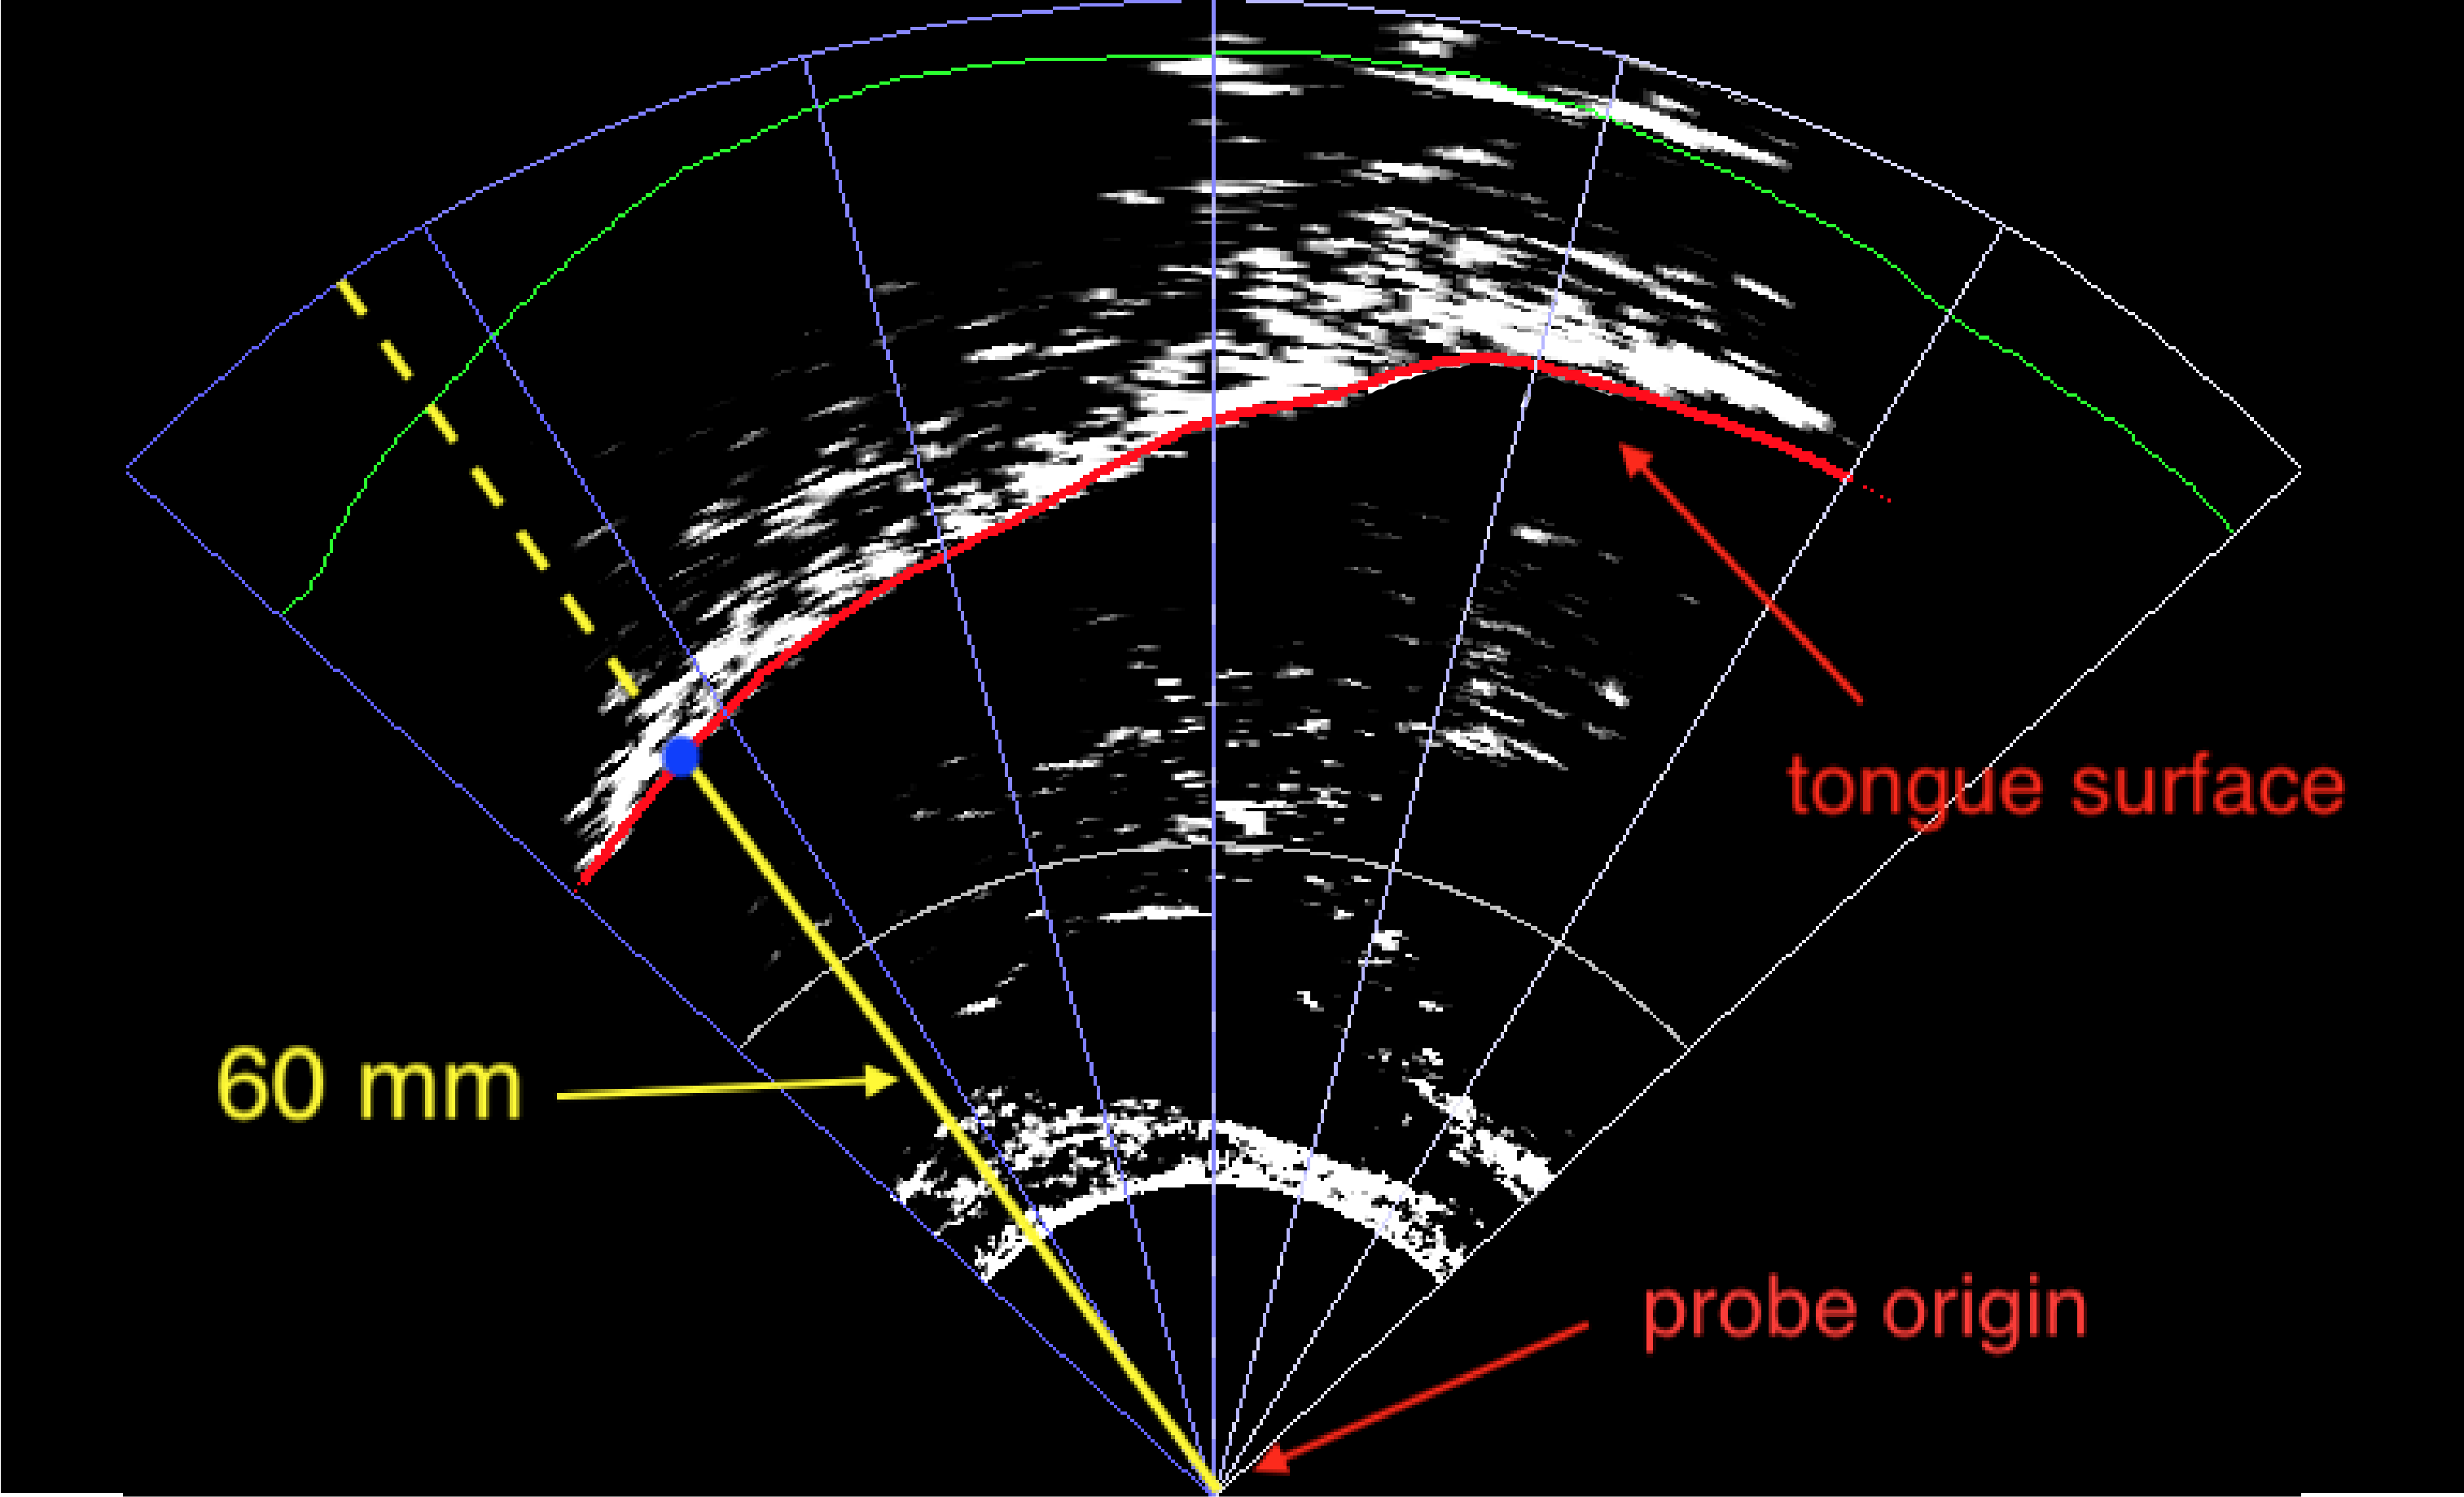
\includegraphics[width=5in]{Figure1.png}
  \caption{Schematics of the operationalisation of tongue root position, based on \citet{kirkham2017}. The tongue root surface corresponds to the lower edge of the white band in the image. The tongue tip is on the right side. The outline of the fan-like coordinate systems is shown. The yellow line starting from the probe origin is the selected fan-line from which tongue root position is calculated (see text for the method of fan-line selection). Tongue root position thus corresponds to the distance (in millimetres) between the probe origin and the intersecting point of the tongue surface with the selected fan-line.}
  \label{f:trp}
\end{figure}

Statistical analysis was performed in R v3.5.2 \citep{r-core-team2018}.
Linear mixed-effects models were fitted with lme4 v1.1-19
\citep{bates2015}. Factor terms were coded with treatment contrasts (the
reference level is the first listed for each factor): C2 voicing
(voiceless, voiced), vowel (/a/, /o/, /u/). Speech rate was centred for
inclusion in the statistical models, by subtracting the mean speech rate
across all speakers from the calculated speech rate values. Centring
ensures the intercepts are interpretable. \emph{t}-tests with
Satterthwaite's approximation to degrees of freedom on the individual
terms were used to obtain \emph{p}-values using lmerTest v3.0-1
\citep{kuznetsova2017, luke2017}. An effect is considered significant if
the \emph{p}-value is below the alpha level (\(\alpha = 0.05\)).
Generalised additive mixed models were fitted with mgcv v1.8-26
\citep{wood2011, wood2017}. The smooths used thin plate regression
splines as basis \citep{wood2003}. The ordered factor difference smooths
method described in \citet{soskuthy2017} and \citet{wieling2018} was
used to model the effect of factor terms in GAMs. The models were fitted
by maximum likelihood (ML) and autoregression in the residuals was
controlled with a first-order autoregressive model.

Significance testing of the relevant predictors was achieved by
comparing the ML score of the full model with the score of a null model
(in which the relevant predictor is dropped), using the
\texttt{compareML()} function of the itsadug package
\citep{van-rij2017}. A preliminary analysis indicated that including
either language or C2 place of articulation as predictors produced
respective \emph{p}-values above the alpha level, without affecting the
estimates of the other terms. \Cref{s:idio} further discusses the
idiosyncratic behaviour of the tongue root observed between speakers,
which does not seem to pattern in any way with their native language.
For these reasons, these variables were not included in the models
reported here and will not be discussed. Future research is warranted to
ascertain language-related differences and possible effects of place of
articulation.

\hypertarget{results}{%
\section{Results}\label{results}}

\label{s:results}

\hypertarget{tongue-root-position-at-c2-closure-onset}{%
\subsection{Tongue root position at C2 closure
onset}\label{tongue-root-position-at-c2-closure-onset}}

\label{s:tra-lm}

\begin{figure}
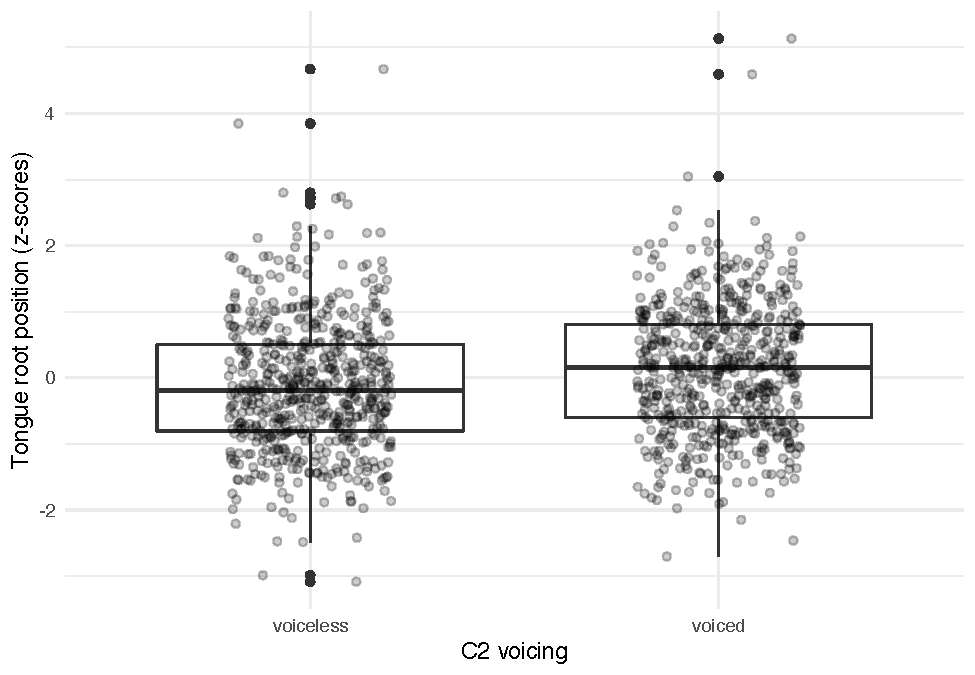
\includegraphics[width=\linewidth]{./Figure2} \caption{Raw data and boxplots of tongue root position in voiceless and voiced stops at closure onset. Higher values indicate advancement.}\label{f:Figure2}
\end{figure}

\Cref{f:Figure2} shows raw data points and boxplots of the position of
the tongue root at C2 closure onset when C2 is voiceless (left) and
voiced (right). Since the position of the tongue root in millimetres
depends on the speaker's anatomy and on the probe location, scaled
tongue root position is used in this plot (note though that the unscaled
data is used in statistical modelling). As a trend, the position of the
tongue root is more advanced if C2 is voiced compared to its position
when C2 is voiceless.

A linear mixed-effects model with tongue root position as the outcome
variable was fitted with the following predictors
(\Cref{tab:tra-lm-table}): fixed effects for C2 voicing (voiceless,
voiced), centred speech rate (as number of syllables per second,
centred), vowel (/a/, /o/, /u/); by-speaker and by-word random
intercepts (a by-speaker random coefficient for C2 voicing led to
singular fit, so it was not included in the final model). The effects of
C2 voicing and vowel are significant according to \emph{t}-tests with
Satterthwaite's approximation to degrees of freedom. The tongue root at
C2 closure onset is 0.77 mm (SE = 0.35) more front when C2 is voiced,
and it is 1.87 mm (SE = 0.42) more retracted if V1 is /o/.

\hypertarget{tongue-root-position-during-v1}{%
\subsection{Tongue root position during
V1}\label{tongue-root-position-during-v1}}

\label{s:trp-v1}

The position of the tongue root during the articulation of V1 was
assessed with generalised additive mixed models (GAMM). A GAMM was
fitted to tongue root position with the following terms
(\Cref{tab:tra-gam-ar-table}): C2 voicing as a parametric term; a smooth
term over centred speech rate, a smooth term over V1 proportion with a
by-C2 voicing difference smooth, a tensor product interaction over V1
proportion and centred speech rate; a factor random smooth over V1
proportion by speaker (penalty order = 1). A chi-squared test on the ML
scores of the full model and a model excluding C2 voicing indicates that
C2 voicing significantly improves fit (\(\chi\)(3) = 7.758, \emph{p} =
0.001). \Cref{f:Figure3} shows that the root advances during the
production of the vowel, relative to its position at V1 onset. This
forward movement is observed both in the context of a following voiced
stop and in that of a following voiceless stop. However, the magnitude
of the movement is greater in the former. At V1 offset (= C2 closure
onset), the graph suggests a difference in tongue root position of about
1 mm.

\begin{figure}
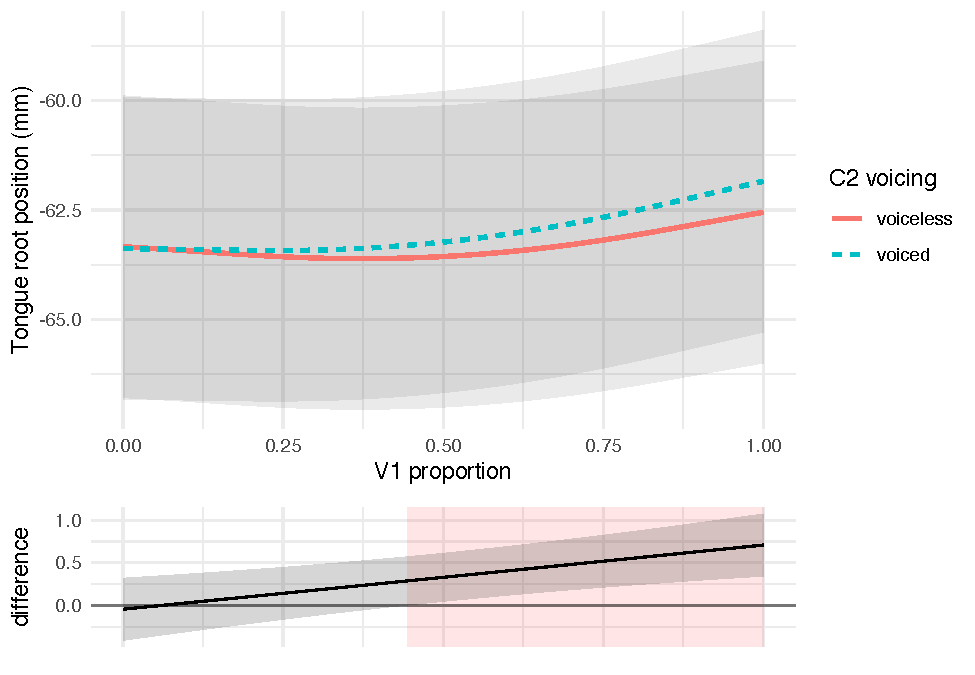
\includegraphics[width=\linewidth]{./Figure3} \caption{Predicted tongue root position (top figure) during vowels preceding voiceless and voiced stops, with 95\% confidence intervals, and difference smooth (bottom figure). Higher values of tongue root position indicate a more advanced root. The shaded red area in the difference smooth indicates where the two curves are different. Predictions from a GAMM (see \Cref{s:trp-v1}).}\label{f:Figure3}
\end{figure}

\hypertarget{correlation-between-tongue-root-position-and-v1-duration}{%
\subsection{Correlation between tongue root position and V1
duration}\label{correlation-between-tongue-root-position-and-v1-duration}}

\label{s:trp-vdur}

\begin{figure}
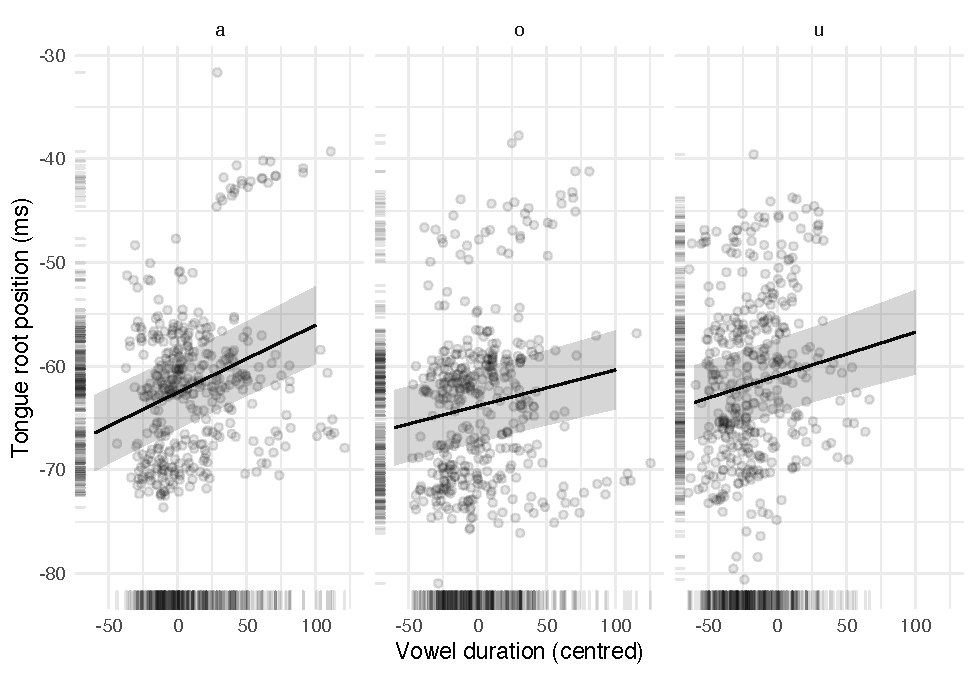
\includegraphics[width=\linewidth]{./Figure4} \caption{Raw data, regression lines, and 95\% confidence intervals of the correlation between vowel duration and tongue root position for each vowel (/a/, /o/, and /u/). The regression line and confidence intervals are from a mixed-effects model (see \Cref{s:trp-vdur}).}\label{f:Figure4}
\end{figure}

A second linear mixed regression was fitted to tongue root position to
assess the effect of V1 duration on root position
(\Cref{tab:tra-lm-2-table}). The following terms were included: centred
V1 duration (in milliseconds), centred speech rate (as number of
syllables per second), vowel (/a/, /o/, /u/), C2 place of articulation
(coronal, velar); an interaction between centred V1 duration and vowel;
by-speaker and by-word random intercept (a by-speaker random coefficient
for V1 duration led to non-convergence, so it was not included in the
final model). All predictors and the V1 duration/vowel interaction are
significant. V1 duration and tongue root position are positively
correlated: The longer the vowel, the more advanced the tongue root is
at V1 offset (\(\hat{\beta}\) = 0.065 mm, SE = 0.007). The effect is
stronger with /a/ than with /o/ and /u/ (see \Cref{f:Figure4}).

\hypertarget{tongue-root-position-during-v1-as-a-function-of-v1-duration}{%
\subsection{Tongue root position during V1 as a function of V1
duration}\label{tongue-root-position-during-v1-as-a-function-of-v1-duration}}

\label{s:trp-v1-dur}

The effect of V1 duration on tongue root position during V1 was modelled
by fitting a GAMM with the following terms
(\Cref{tab:tra-gam-ar-2-table}): tongue root position as the outcome
variable, smooth terms over V1 duration and V1 proportion, a tensor
product interaction over V1 proportion and V1 duration; a factor random
smooth over V1 proportion by speaker (penalty order = 1). The full model
with the tensor product interaction over V1 proportion and V1 duration
has better fit according to model comparison with a model without the
interaction (\(\chi\)(3) = 12.559, \emph{p} \textless{} 0.001).
\Cref{f:Figure5} shows the estimated root trajectories at four values of
vowel duration. The general trend is that the forward movement of the
root during the vowel is greater the longer the duration of the vowel
(\Cref{f:Figure5}). Moreover, the trajectory curvature increases with
vowel duration: Shorter vowels have a flatter trajectory of tongue root
advancement.

\begin{figure}
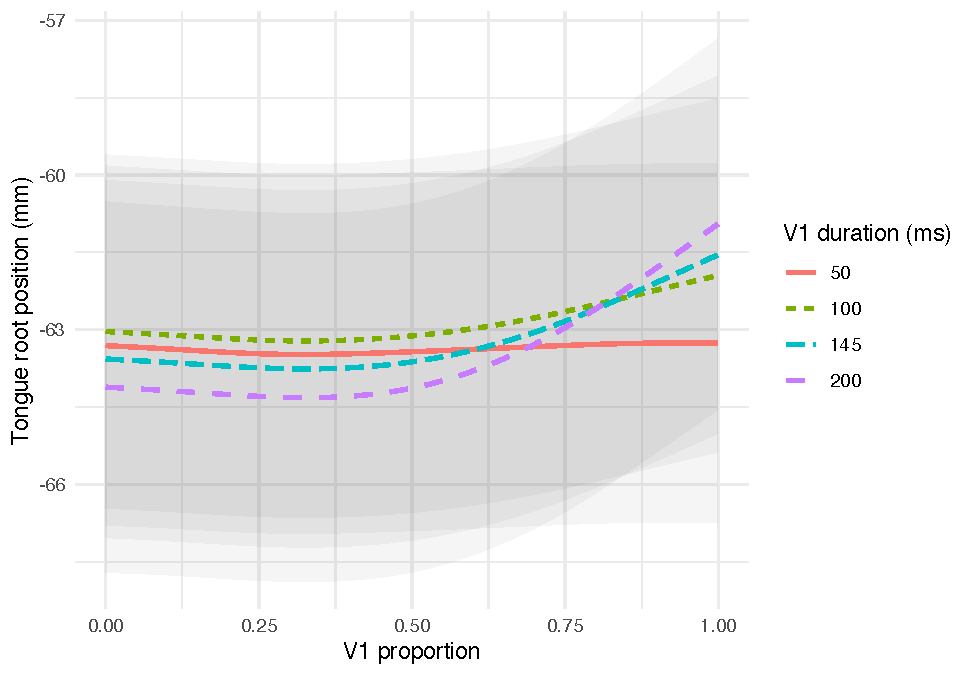
\includegraphics[width=\linewidth]{./Figure5} \caption{Predicted tongue root position during vowels at 4 exemplifying values of vowel duration, with 95\% confidence intervals. Predictions from a GAMM (see \Cref{s:trp-v1-dur}).}\label{f:Figure5}
\end{figure}

\hypertarget{discussion}{%
\section{Discussion}\label{discussion}}

\label{s:discussion}

\hypertarget{voicing-tongue-root-position-and-vowel-duration}{%
\subsection{Voicing, tongue root position and vowel
duration}\label{voicing-tongue-root-position-and-vowel-duration}}

The results of this study of voicing and vowel duration in Italian and
Polish revealed a few patterns in the relation between consonant
voicing, tongue root position, and vowel duration. Unsurprisingly, the
position of the tongue root at vowel offset is more front when the
following stop is voiced than when the following stop is voiceless in
both surveyed languages. This finding aligns with the results of
previous work on English
\citep{kent1969, perkell1969, westbury1983, ahn2018}. When looking at
the position of the tongue root during the vowel, it was found that the
root starts advancing during the articulation of the vowel.
\citet{westbury1983} found the same pattern in English. Moreover,
similarly to the results in \citet{westbury1983}, some tongue root
advancement during the production of the vowel is found even when C2 is
voiceless.

A possible reason for the presence of such a small degree of advancement
in voiceless lingual stops is offered by arguments in relation to the
absence of advancement in labials (voiced or voiceless).
\citet{westbury1983} proposes that the articulation of the closure of
lingual stops mechanically involves movements of the tongue root, so
that, in order to keep a constant oral cavity volume, the root moves
forward while the tongue body moves upward. On the other hand, the
tongue can move freely in labial stops since their closure involves the
lips. This idea is supported by the `trough effect'
\citep{vazquez-alvarez2007}, i.e.~VCV sequences involving a labial stop
show tongue body lowering, and by the fact that voiced labials tend to
resort to tongue body lowering rather than tongue root advancement as a
mechanism for voicing maintenance
\citep{perkell1969, westbury1983, ahn2018}. The small degree of
advancement in voiceless lingual stops could then as well be a mechanic
consequence of the tongue moving upward for producing the stop closure.

The data discussed here also suggest that tongue root position is
positively correlated with vowel duration, such that longer vowels show
a more advanced tongue root at vowel offset (= closure onset) than
shorter vowels. Said correlation exists independent of the voicing
status of the consonant following the vowel (compatible with the finding
that even voiceless stops have some degree of advancement). The
correlation between tongue root and vowel duration could be interpreted
as to indicate that the onset of the forward gesture of the root is
timed relative to a landmark preceding the closure, independent of the
duration of the vowel. The timing of the stop closure along the
advancement movement would sanction the degree of advancement found at
closure onset.

The dynamic data of tongue root advancement during the articulation of
the vowel indicates that vowels followed by voiced stops have greater
tongue root advancement at vowel offset than vowels followed by
voiceless stops, in accordance with the results from the static analysis
at vowel offset. Moreover, a significant interaction between vowel
duration and the trajectory shape was found. Shorter vowels have a
flatter trajectory, while the curvature of the trajectory in longer
vowels has a greater curvature.

When comparing the effects of vowel duration and speech rate on tongue
root position, though, we are faced with a paradox. Both variables have
a positive effect on tongue root position, so that longer vowels and
higher speech rates imply a more advanced root. However, speech rate has
a negative effect on vowel duration (and segments duration in general),
such that higher speech rates are correlated with shorter vowel
durations (this holds for this data). If higher speech rates mean
shorter vowels and shorter vowels imply a less advanced root, we should
also find less advancement with higher speech rates. However, the
results indicate the opposite, and higher speech rates are correlated
with more root advancement. However, a regression model on the position
of the tongue root at \emph{vowel onset} suggests that speech rate is
positively correlated with tongue root position at vowel onset. The
tongue root is already in a more advanced position at vowel onset when
the speech rate is high, so that, if vowel duration is held constant,
more advancement is expected at vowel offset with higher speech rates
even when higher speech rate has a negative effect on vowel duration.

The articulatory patterns observed in this paper contribute to the
understanding of the acoustic patterns discussed in previous work. If we
take the release of the consonant preceding the vowel as a reference
point, a delayed consonant closure could ensure that, by the time
closure is made, an appreciable amount of tongue root advancement is
achieved. Other things being equal, an increase in cavity volume
increases the time required to reach trans-glottal pressure
equalisation, which would cause cessation of voicing. This mechanism
thus contributes to the maintenance of voicing during the stop closure.

The closure of voiced stops is achieved later (relative to the preceding
consonant release) compared to the closure of voiceless stops. Moreover,
the temporal distance between the releases of the two consecutive stops
in CV́CV words is not affected by the voicing category of the second
stop. Given the stability of the release to release interval duration,
the delay in producing a full closure seen in the context of voiced
stops has thus a double advantage: (1) A greater degree of tongue root
advancement is achieved at vowel offset/closure onset, and (2) the stop
closure is shorter. Both of these articulatory features are compliant
with the requirements dictated by the aerodynamic voicing constraint. A
more advanced tongue root ensures that the trans-glottal pressure
differential is sufficient for voicing to be sustained, and a shorter
closure reduces the pressure build-up during the stop closure. To
conclude, it is proposed that the combined action of a temporally stable
release to release interval and the differential timing of the VC
boundary in the context of voiceless vs.~voiced stops contribute to both
the acoustic patterns of vowel and closure duration and the articulatory
patterns of tongue root position.

\hypertarget{estimates-of-tongue-root-displacement}{%
\subsection{Estimates of tongue root
displacement}\label{estimates-of-tongue-root-displacement}}

It is worth to briefly discuss the estimated difference in tongue root
position between voiceless and voiced stops and its significance. The
estimated magnitude of such difference is 0.77 mm (SE = 0.35). The 95\%
confidence interval for the difference is approximately within the range
0-1.5 mm. \citet{rothenberg1967} argues that the anterior wall of the
lower pharynx (corresponding to the tongue root) can move by 5 mm along
the antero-posterior axis. Figure 1 in \citet{kirkham2017} suggests that
the tongue root of one of the Twi speakers recorded is about 4 mm more
front in /e/ (a +ATR vowel) than in /ɛ/ (a -ATR vowel). Given that a
difference of 4 mm in root position can produce a substantially distinct
acoustic output in vowels (like the two different phonemes of Twi), it
makes sense to expect that differences in tongue root position as driven
by consonantal factors should be of some magnitude smaller, like the
once found in this study. Moreover, the data presented here indicates
that for every millisecond increase in vowel duration there is a 0.065
mm increase in tongue root advancement (see \Cref{s:trp-vdur}). If a
maximal ballistic forward movement of the tongue root takes between 70
and 90 ms \citep{rothenberg1967}, we can calculate the maximum
displacement plausible to be between 4.55 to 5.85 mm (0.065 mm times
70--90 ms). These values are in agreement with the maximum root
displacement of 5 mm estimated by Rothenberg.

The results of this study also shed some light on timing aspects of
tongue root advancement. As mentioned in the previous section, the
correlation between tongue root position and vowel duration could be a
consequence of the timing of the advancement gesture. In order to obtain
such correlation, the onset of the gesture (during the articulation of
the vowel) should be at a fixed distance from an earlier reference point
(like the vowel onset or the preceding consonant offset) such that the
timing of consonant closure will create the correlation seen in the
data. Although ideally the timing of the onset of the advancing gesture
should be fixed, the velocity of the gesture itself could be different
depending on the voicing of the following consonant. It is possible that
the velocity will be greater in the context of voiced stops, especially
if the advancing gesture in this context is executed with greater
muscular force. Unfortunately, a preliminary screening of the current
data was inconclusive as to whether timing and velocity are similar or
differ in the voiceless and voiced contexts, due to the difficulty in
identifying the onset of the advancing gesture. Further data should be
collected with the aim of testing the hypothesis that the timing of the
gesture onset is the same in voiceless and voiced contexts, while the
velocity of the gesture should differ.

Although the results of this study are in agreement with previous work,
the correlation between tongue root position and vowel duration needs to
be replicated by expanding the enquired contexts to other types of
consonants and vowels, and with other languages. Investigating the
relative phasing of tongue root and body gestures in lingual and labial
consonants is also necessary to clarify the mechanisms that could
underlie the gestural timing of stop closure and tongue root
advancement. Moreover, while the paper so far has focussed on
group-level trends, it should be noted that, as found in other studies
on the tongue root, individual speakers show a somewhat high degree of
variability. The following section discusses this point.

\hypertarget{individual-differences}{%
\subsection{Individual differences}\label{individual-differences}}

\label{s:idio}

\begin{figure}

{\centering 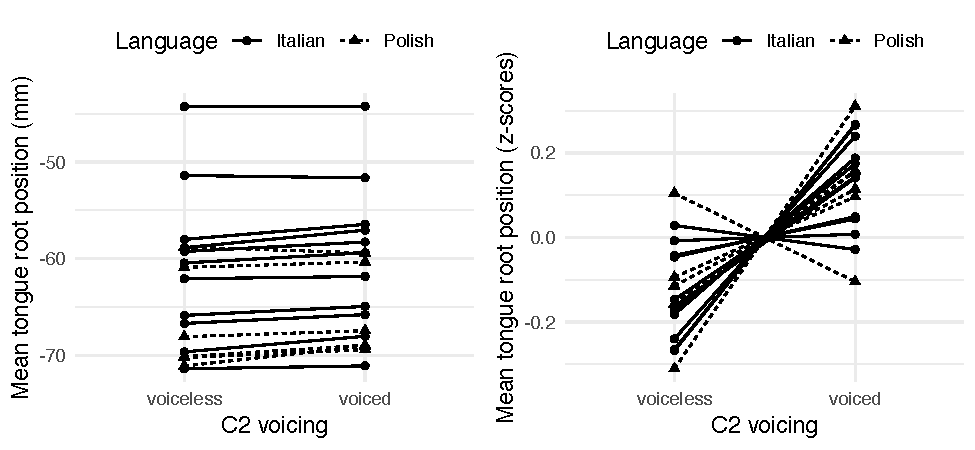
\includegraphics[width=\linewidth]{./Figure6} 

}

\caption{Slope plots of mean torngue root position in voiceless and voiced stops at closure onset, by-speaker. The plot on the left has raw position values in millimetres, while the plot on the right shows standardised values (z-scores) by speaker. See text for details.}\label{f:Figure6}
\end{figure}

The results presented in \Cref{s:results} and discussed in
\Cref{s:discussion} are group-level patterns of the population sampled
in the present study. However, the data is characterised by a certain
degree of individual-level differences. \Cref{f:Figure6} shows two slope
plots of mean tongue root position depending on C2 voicing for each
speaker. In each plot, the two means of each speaker are linked by a
line that shows the difference (or lack thereof) in means. Solid lines
are Italian speakers, while dashed lines are Polish speakers. The
\emph{y}-axis of the left plot is the raw mean position in millimetres,
while that of the right plot is the standardised values (z-scores) of
the mean position. An upward-slanted slope line indicates that the mean
tongue root position in the voiced condition is higher, while a
downward-slanted slope is interpreted as a decrease in mean root
position. A flat slope suggests there is no difference in means between
the voiceless and voiced condition.

This plot show that all three possibilities of slope direction are found
in the data. The mean value of tongue root position of a voiced C2
relative to that of a voiceless stop is greater in some speakers,
smaller in others, and similar in yet other speakers. Moreover, no
discernible pattern can be found between speakers of Italian and Polish.
Speakers of both languages show more or less the same range of
variation. However, as we have seen in \Cref{s:results}, the estimated
overall effect of C2 voicing is robust and it implies a more advanced
tongue root in voiced stops. The right plot of \Cref{f:Figure6} confirms
this point visually. Two speakers show a declining slope (one is Italian
and the other Polish), one speaker has a virtually flat slope, while all
the others have an increasing slope at varying degrees. Note that the
individual variation across speakers found in this data is qualitatively
comparable to that in \citet{ahn2018}.

\begin{figure}
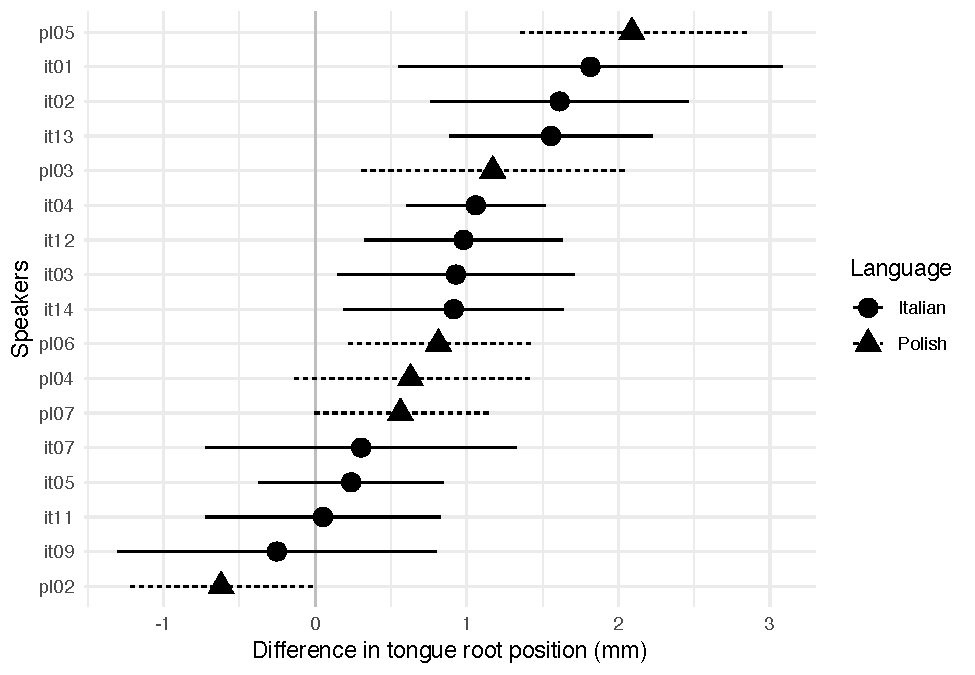
\includegraphics[width=\linewidth]{./Figure7} \caption{By-speaker raw mean difference in tongue root position between voiceless and voiced stops at closure onset (in millimetres). The horizontal segments are the standard errors of the mean differences.}\label{f:Figure7}
\end{figure}

The mean difference in tongue root position in voiceless vs.~voiced
stops has been calculated for each speaker from the raw data.
\Cref{f:Figure7} plots the speakers' mean differences, with the
respective standard error bars. The bottom 7 speakers (3 Polish, 4
Italian) show either a weak negative difference (the tongue root is
slightly more advanced in voiceless stops) or a weak positive difference
with wide standard errors which include 0. The remaining 11 speakers
have a more robust positive difference (the tongue root is more advanced
in voiced stops). Finally, speakers of each language do not cluster
together, reiterating the observation made above that language does not
seem to be an informative parameter.

Finally, interesting individual patterns can also be seen in the
trajectories of tongue root position. \Cref{f:Figure8} shows these
trajectories for all the speakers (note that the \emph{y}-axis of each
plot is on a different scale, so magnitude comparisons should not be
made visually). Speakers IT01, IT03, and PL04 in particular have a
somewhat categorical distinction in tongue root position during vowels
followed by voiceless vs.~voiced stops. Such tongue root distinction is
implemented across the total duration of the vowel, rather than towards
the end (as suggested by the results from the aggregated data, see
\Cref{s:trp-v1}). The phonological literature reports cases in which the
difference in tongue root position in vowels is enhanced, leading to
phonological alternations or diachronic loss of the voicing distinction
with maintenance of the tongue root distinction (see \citealt{vaux1996}
and references therein). The ultrasound data from this study offers
articulatory evidence for a possible precursor of said phonological
patterns.\footnote{All the examples in \citet{vaux1996} are on vowels \textit{following} voiceless vs. voiced stops, rather than preceding, as in the current study. While beyond the scope of this paper, whether this is a systematic gap or not and how this relates to the present findings should be examined in future work.}

\begin{figure}
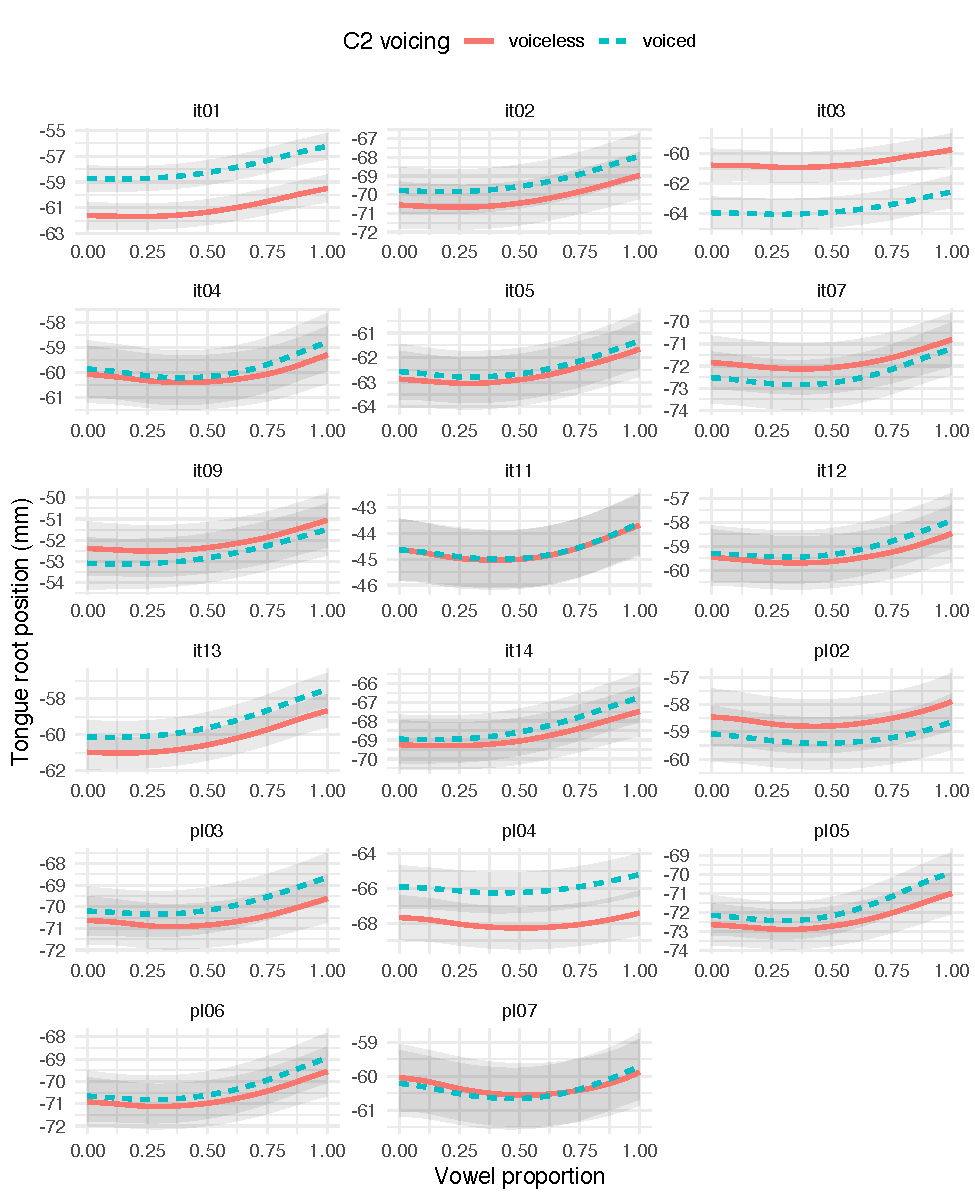
\includegraphics[width=\linewidth]{./Figure8} \caption{Predicted tongue root position during vowels followed by voiceless and voiced stops for each speaker. Predicted from a GAMM (see text). Note the different scales on the y-axis.}\label{f:Figure8}
\end{figure}

\hypertarget{conclusion}{%
\section{Conclusion}\label{conclusion}}

The maintenance of voicing during the closure of stops can achieved
through a variety of articulatory mechanisms. Among these, shorter
closure durations and cavity expansion by tongue root advancement are
commonly observed solutions. Another robust correlate of consonant
voicing is longer preceding vowel duration. This paper discussed
articulatory data from an exploratory study of the effect of voicing on
vowel duration first introduced in \citet{coretta2018j}. Similarly to
what previously found for English, the tongue root at stop closure onset
is more advanced in voiced than in voiceless stops in Italian and
Polish. The average difference in tongue root position is 0.77 mm (SE =
0.35). By modelling the trajectory of the tongue root during the
production of vowels preceding stops, it was found that the root starts
advancing during the vowel, both preceding voiceless and voiced stops.
The magnitude of the advancing gesture was however greater in the voiced
context. Moreover, tongue root position and vowel duration were found to
be positively correlated. Longer vowel durations correspond to greater
tongue root advancement.

It was argued that the combined action of two factors contribute to the
patterns observed: (1) The duration of the interval between two
consecutive releases, and (2) the timing of the C2 closure onset within
such interval. The release to release interval duration has been found
not to be affected by the voicing of the second consonant. The later
closure onset of voiced stops within the release to release interval
(compared to voiceless stops) has the double advantage of producing a
shorter closure duration and ensuring that enough tongue root
advancement is reached by the time the stop closure is achieved. Both of
these aspects comply with the aerodynamic voicing constraint
\citep{ohala2011} by delaying trans-glottal pressure equalisation (which
would prevent vocal fold vibration). Future studies will need to test
whether these findings replicate in Italian and Polish, and if they
extend to other languages and contexts. In particular, further work on
the relative differences in timing and velocity of the closing gesture
and the root advancement gesture will be necessary to obtain a more
in-depth understanding of the relation between consonant voicing, tongue
root position, and vowel duration.

\appendix

\hypertarget{target-words}{%
\section{Target words}\label{target-words}}

\label{a:targets}

See \Cref{t:targets}.

\ctable[caption = The list of Italian and Polish target words. An asterisk indicates a real word.,
label = t:targets,
star,
doinside = \footnotesize
]{lllllll}{}{
\FL
Italian   &        &      & \hspace{0.5cm} & Polish &      &      \NN
\cmidrule{1-3}\cmidrule{5-7}
pata      & poto*  & putu & & pata   & poto & putu \NN
pada      & podo   & pudu & & pada*  & podo & pudu \NN
paca*     & poco*  & pucu & & paka*  & poko & puku \NN
paga*     & pogo   & pugu & & paga   & pogo & pugu \LL
}

\hypertarget{output-of-statistical-models}{%
\section{Output of statistical
models}\label{output-of-statistical-models}}

See \Cref{tab:tra-lm-table}, \Cref{tab:tra-gam-ar-table},
\Cref{tab:tra-lm-2-table}, \Cref{tab:tra-gam-ar-2-table}.

\begin{table}[t]

\caption{\label{tab:tra-lm-table}Summary of the linear mixed-effects model fitted to tongue root position at vowel offset (see \Cref{s:tra-lm})}
\centering
\fontsize{10}{12}\selectfont
\begin{tabular}{lrrrrrrrl}
\toprule
Predictor & Estimate & SE & CI low & CI up & df & t-value & p-value & < α\\
\midrule
Intercept & -62.1396 & 1.8113 & -65.6898 & -58.5895 & 17.1188 & -34.3058 & 0.0000 & *\\
Voicing = voiced & 0.7689 & 0.3473 & 0.0881 & 1.4497 & 19.3947 & 2.2137 & 0.0390 & *\\
Speech rate (centr.) & 0.4114 & 0.2793 & -0.1360 & 0.9588 & 1168.1100 & 1.4732 & 0.1410 & \\
Vowel = /o/ & -1.8742 & 0.4249 & -2.7069 & -1.0414 & 19.2874 & -4.4112 & 0.0003 & *\\
Vowel = /u/ & 0.0865 & 0.4270 & -0.7503 & 0.9233 & 19.6974 & 0.2027 & 0.8415 & \\
\bottomrule
\end{tabular}
\end{table}

\begin{table}[t]

\caption{\label{tab:tra-gam-ar-table}Summary of the GAM model fitted to tongue root position during V1 (see \Cref{s:trp-v1})}
\centering
\fontsize{10}{12}\selectfont
\begin{tabular}{lrrrrrrl}
\toprule
Predictor & Estimate & SE & EDF & Ref.DF & Statistic & p-value & < α\\
\midrule
Intercept & -63.3328 & 1.7562 &  &  & -36.0623 & 0.0000 & *\\
Voicing = voiced & 0.3311 & 0.1432 &  &  & 2.3122 & 0.0208 & *\\
s(Speech rate (centr.)) &  &  & 7.5311 & 8.5159 & 4.4779 & 0.0000 & *\\
s(Proportion) &  &  & 3.6915 & 4.3646 & 10.4427 & 0.0000 & *\\
s(Proportion): voiced &  &  & 1.0122 & 1.0236 & 10.0413 & 0.0015 & *\\
ti(Proportion, Speech Rate (c.)) &  &  & 2.1335 & 2.7679 & 2.9005 & 0.0429 & *\\
s(Proportion, Speaker) &  &  & 62.2821 & 152.0000 & 57.3445 & 0.0000 & *\\
\bottomrule
\end{tabular}
\end{table}

\begin{table}[t]

\caption{\label{tab:tra-lm-2-table}Summary of the linear mixed-effects model for testing the correlation between tongue root position and V1 duration  (see \Cref{s:trp-vdur})}
\centering
\fontsize{10}{12}\selectfont
\begin{tabular}{lrrrrrrrl}
\toprule
Predictor & Estimate & SE & CI low & CI up & df & t-value & p-value & < α\\
\midrule
Intercept & -62.5793 & 1.7818 & -66.0716 & -59.0870 & 17.0874 & -35.1212 & 0.0000 & *\\
V1 duration (centr.) & 0.0651 & 0.0073 & 0.0507 & 0.0795 & 955.6436 & 8.8558 & 0.0000 & *\\
Speech rate (centr.) & 1.2412 & 0.2903 & 0.6722 & 1.8102 & 1169.6885 & 4.2755 & 0.0000 & *\\
Vowel = /o/ & -1.3031 & 0.4597 & -2.2040 & -0.4021 & 18.3761 & -2.8348 & 0.0108 & *\\
Vowel = /u/ & 1.5863 & 0.5049 & 0.5967 & 2.5759 & 25.8255 & 3.1419 & 0.0042 & *\\
V1 duration × /o/ & -0.0303 & 0.0079 & -0.0457 & -0.0149 & 736.2314 & -3.8504 & 0.0001 & *\\
V1 duration × /u/ & -0.0227 & 0.0090 & -0.0403 & -0.0052 & 751.2493 & -2.5345 & 0.0115 & *\\
\bottomrule
\end{tabular}
\end{table}

\begin{table}[t]

\caption{\label{tab:tra-gam-ar-2-table}Summary of the GAM model fitted to tongue root position during V1 as a function of V1 duration (see \Cref{s:trp-v1-dur})}
\centering
\fontsize{10}{12}\selectfont
\begin{tabular}{lrrrrrrl}
\toprule
Predictor & Estimate & SE & EDF & Ref.DF & Statistic & p-value & < α\\
\midrule
Intercept & -63.0628 & 1.7397 &  &  & -36.2487 & 0 & *\\
s(V1 duration) &  &  & 8.2416 & 8.8458 & 7.7094 & 0 & *\\
s(Proportion) &  &  & 3.9640 & 4.7069 & 17.9941 & 0 & *\\
ti(Proportion, V1 duration) &  &  & 2.8557 & 3.3236 & 8.9785 & 0 & *\\
s(Proportion, Speaker) &  &  & 59.9588 & 152.0000 & 65.7394 & 0 & *\\
\bottomrule
\end{tabular}
\end{table}

%% before appendix (optional) and bibliography:
% \begin{acknowledgments}
%This research was supported by  ...
% \end{acknowledgments}

% -------------------------------------------------------------------------------------------------------------------
%   Appendix  (optional)

%\appendix
%\section{Appendix title}

%If only one appendix, please use
%\appendix*
%\section{Appendix title}


%=======================================================
%IMPORTANT

%Use \bibliography{<name of your .bib file>}+
%to make your bibliography with BibTeX.

%Once you have used BibTeX you
%should open the resulting .bbl file and cut and paste the entire contents
%into the end of your article.
%=======================================================

\bibliography{linguistics}


\end{document}
